\documentclass[table]{elegantpaper}
\usepackage{datetime2}
\usepackage[T1]{fontenc}
\usepackage{graphicx}
\usepackage{listings}
\usepackage{listings-rust}
\usepackage{pgf-pie}
\usepackage{rotating}
\usepackage{tabularray}
\usepackage{tabularx}
\usepackage{xcolor}

\DTMusemodule{english}{en-GB}
\DTMnewdatestyle{short}{
  \renewcommand{\DTMdisplaydate}[4]{
    \DTMenglishmonthname{##2} \number##1\relax
  }
  \renewcommand{\DTMDisplaydate}{\DTMdisplaydate}
}
\newcommand{\shorttoday}{{\DTMsetdatestyle{short}\today}}
\renewcommand{\updatetext}{}

\graphicspath{{./images/}}
\DeclareEmphSequence{\bfseries,\itshape,\upshape}
\lstset{xleftmargin=\parindent,xrightmargin=\parindent}

\title{Groth16 Implementment Specification in BitVM2}
\author{Fiamma \thanks{\url{https://twitter.com/Fiamma_Chain}}}
\date{\shorttoday}

\addbibresource[location=local]{reference.bib}

\begin{document}
    \maketitle
    \begin{abstract}
    In this paper, we will show how we implement the Groth16 verification in Bitcoin, we are grateful to all the members who contribute to BitVM2 repository,
    such as Robin, Weikeng, and Zerosync team, etc. Based on this paper, we hope:
    (1). Our design and implementment could be reviewed by BitVM2 community;
    (2). Let more developer and researchers to know the details that how BitVM2 works with Groth16;
    (3). Accelerating the process of BitVM2 with whole community to ensure it could be adopted in production in a safe way;
\end{abstract}

    \tableofcontents
    \section{The Basics} \label{sec:the-basics}
The section will introduce some basic knowledgers you would better to know, including 
(1). The Groth16 verification progress;
(2). On proving pairing;
(3). Limitations when split the script;

\subsection{Groth16-verification-program}

The blockchain industry has seen a tremendous pace of development over the past few years, exploring applications and opportunities built on these systems. With this rapid expansion, the industry faces a major technical challenge in improving processing capacity of the blockchain to achieve higher throughput while still maintaining its security. Currently, some very prominent teams have made great progress to achieve this, such as PSE \cite{website:pse}, Matter Labs \cite{website:matter-labs}, Polygon Hermez \cite{website:hermez}, StarkWare \cite{website:starkware}, Risc0 \cite{website:risc0} and Scroll \cite{website:scroll}.

We are able to divide the above mentioned projects into three different levels based on differences in their compatibility with EVM: Consensus-level, Bytecode-level, and Language-level.

First up is PSE, that has a Consensus-level compatibility with EVM, meaning it is fully compatible with EVM. The ZK constraints are consistent with the current behaviour of EVM, this includes the update of the state root, which is advantageous in that you only need to design the circuit to constrain all the rows of EVM. Secondly, Scroll and Polygon has a Bytecode-level compatibility with EVM, which directly interprets the bytecode of EVM, whilst using a different account model to increase ZK efficiency, resulting in different state roots. The advantage of this is that the compatibility with EVM is still guaranteed and the proof efficiency of state root is improved. Due to the introduction of different account models, additional changes at EVM level are required compared to a Consensus-level scheme. Last up is Language-level compatibility, utilized by projects such as StarkWare, Matter Labs and Risc0. They define a ZK-friendly VM, which includes a custom instruction set, custom memory model and so on. They convert Solidity (or Yul) into custom VM-supported instructions through a compiler. The advantage of this solution is achieving that allows for deploying most contracts directly without modification and at the same time providing the highest ZK efficiency in its smaller execution traces and simple state transition constraints. However, trade-offs lie in huge workloads involving constraint design, VM design and compiler design, amongst others. Following we will briefly introduce the general framework of the three mentioned schemes.

\subsubsection{Consensus-level Compatibility}

The main advantage of this scheme is that it maintains full compatibility to the current behaviour of EVM. All behaviors of EVM are constrained by circuits, including but not limited to memory access, instruction execution, and world state updates. Execution traces are generated by EVM Runner, then it is generating a proof that EVM produces combined with its corresponding ZK constraint. The framework of this scheme is shown in Figure \ref{fig:zkevm-architecture-consensus-level}.
\begin{figure}[!ht]
    \centering
    \includegraphics[width=0.8\textwidth]{zkevm-architecture-consensus-level.jpg}
    \caption{ZKEVM architecture based on Consensus-level}
    \label{fig:zkevm-architecture-consensus-level}
\end{figure}

The main workload of this scheme lies in the design of ZK constraints which does not require any modifications to EVM. Which is advantageous, but it is also disadvantageous because there are ZK-unfriendly operations in EVM that also must be proven by ZK-constraints, which makes the overall ZK efficiency low.

\subsubsection{Bytecode-level Compatibility}

Intuitively you may assume that the feature of this scheme is that it can process all the instructions of EVM on Bytecode-level (That the bytecodes of a Solidity contract can be directly used as input), however, other parts than the instructions can be different, such as getting a different state root and using a different hash algorithm. The framework of the scheme is shown in Figure \ref{fig:zkevm-architecture-bytecode-level}.
\begin{figure}[!ht]
    \centering
    \includegraphics[width=0.8\textwidth]{zkevm-architecture-bytecode-level.jpg}
    \caption{ZKEVM architecture based on Bytecode-level}
    \label{fig:zkevm-architecture-bytecode-level}
\end{figure}

As you can tell by this scheme it requires designing or modifying the VM in addition to designing ZK constraints. As an example, Scroll may only need to make corresponding modifications based on the Ethereum client, but Hermez is slightly more complicated due to them customizing a VM. Compared with the Consensus-level ZKEVM scheme, the ZK efficiency of this scheme is slightly better.

\subsubsection{Language-level Compatibility}

Compared to previous two schemes, Language-level compatibility is the weakest. It does not have to be 100\% compatible with EVM, which means that simple modifications to some contracts could result in it needing a lot of support. However, the overall scheme has a ZK-friendly design, e.g, the memory model, instruction set, account model and so on, hence it has a better ZK efficiency. The framework of this scheme is shown in Figure \ref{fig:zkevm-architecture-language-level}.
\begin{figure}[!ht]
    \centering
    \includegraphics[width=0.8\textwidth]{zkevm-architecture-language-level.jpg}
    \caption{ZKEVM architecture based on Language-level}
    \label{fig:zkevm-architecture-language-level}
\end{figure}

Out of all the schemes this has the highest workload, involving the compiler, VM \& constraint design and so on. However, it is also achieving the best ZK efficiency. An example would be StarkWare's Cairo VM, which has a surprisingly good performance in terms of capacity expansion. StarkWare team has come quite far with the Cairo design in terms of being ZK-friendly since the inception of teams pursuing developing a ZKEVM solution.

\subsection{On-proving-pairing}

This is a efficient ways to prove correctness of elliptic curve pairing relations, the algorithm shows in page 25:

Algorithm 9: Multi Miller loop with embedded $c$ exponentiation 

Input: $\displaystyle A = [(P_1,Q_1), (P_2,Q_2),...,(P_n,Q_n)],c, c^{-1} \in F_{q^k},s \in F_{q^3},P_{Q_j} \leftarrow \mathcal{L}(Q_j)$ 

Output: $\displaystyle 1 \ \ if \prod_{i=0}^{n}e(P_i, Q_i) = 1 $ 

(1) assert $\displaystyle c \cdot c^{-1} = 1 $ 

(2) $\displaystyle f \leftarrow c^(-1), lc \leftarrow 0 $ 

(3) Initialize array $T$ such that $\displaystyle T[j] = Q_j $ for each non-fixed point $Q_j$ 

(4) for $i$ = $L-2$ to $0$ do 

(5) \indent $f$ = $f^2$ 

(6) \indent for j=1 to n do 

(7) \indent \indent $\displaystyle l \leftarrow P_{Q_j}[lc] $ 

(8) \indent \indent $\displaystyle f = f \cdot l.evaluate(P_j) $  

(9) \indent \indent if $Q_j$ is not fixed then 

(10) \indent \indent \indent $\displaystyle T \leftarrow T[j] $ 

(11) \indent \indent \indent assert $\displaystyle l.is_tangent(T) $ 

(12) \indent \indent \indent $\displaystyle T[j] = l.double(T) $ 

(13) \indent \indent end 

(14) \indent \indent if $bit^2 == 1$ then 

(15) \indent \indent \indent $\displaystyle f = f \cdot c^{-1}$ if $bit$ == 1 else $\displaystyle f \cdot c$ end 

(16) \indent \indent \indent $\displaystyle l \leftarrow P_{Q_j}[lc+1] $ 

(17) \indent \indent \indent $\displaystyle f = f \cdot l.evaluate(P_{j})$ 

(18) \indent \indent \indent if $Q_j$ is not fixed then 

(19) \indent \indent \indent \indent $\displaystyle Q^{'} = Q_j $ if $bit$ == 1 else $\displaystyle -Q_j $ 

(20) \indent \indent \indent $\displaystyle T \leftarrow T[j] $ 

(21) \indent \indent \indent assert $\displaystyle l.is_line(T, Q^{'}) $ 

(22) \indent \indent \indent $\displaystyle T[j] = l.add(T, Q^{'}) $ 

(23) \indent \indent \indent end 

(24) \indent \indent end 

(25) \indent end 

(26) \indent $\displaystyle lc = lc + 2 $ 

(27) \indent for j=0 to n do 

(28) \indent \indent $\displaystyle f \leftarrow f \cdot s \cdot (c^{-1})^q \cdot (c^{-1})^{q^2} \cdot (c^{-1})^{q^3} $ 

(29) \indent \indent $\displaystyle l_{1..3} \leftarrow (P_{Q_j}[lc+i])_{i=0}^2 $ 

(30) \indent \indent $\displaystyle f \leftarrow f \cdot l_1.evaluate(P_{j}) \cdot l_2.evaluate(P_{j}) \cdot l_3.evaluate(P_{j}) $ 

(31) \indent \indent if $Q_j$ is not fixed then 

(32) \indent \indent \indent $\displaystyle Q_1 \leftarrow \pi_p(Q), Q_12\leftarrow \pi_p(Q_1), Q_3 \leftarrow \pi_p(Q_2) $ 

(33) \indent \indent \indent $\displaystyle T \leftarrow T[j] $ 

(34) \indent \indent \indent assert $\displaystyle l_1.is_line(T, Q_1); T \leftarrow T + Q_1 $ 

(35) \indent \indent \indent assert $\displaystyle l_2.is_line(T, -Q_2); T \leftarrow T - Q_1 $ 

(36) \indent \indent \indent assert $\displaystyle l_3.is_line(T, Q_3) $ 

(37) \indent \indent end 

(38) \indent end 

(39) end 

(40) return $\displaystyle f == 1? $ 


if We adopt this algorithm into Groth16, The whole algorithm process should be like this:

$\displaystyle P_1 = [msm]_1; Q_1 = -[\gamma]_2 $

$\displaystyle P_2 = [C]_1; Q_2 = -[\delta]_2 $

$\displaystyle P_3 = [\alpha]_1; Q_3 = -[\beta]_2 $

$\displaystyle P_4 = [A]_1; Q_4 = [B]_2 $


$Q_4$ is non-fixed, $Q_1$, $Q_2$, and $Q_3$ is fixed.


Input: $\displaystyle A = [(P_1,Q_1), (P_2,Q_2), (P_3,Q_3),(P_4,Q_4)],c, c^{-1} \in F_{q^k},s \in F_{q^3},P_{Q_4} \leftarrow \mathcal{L}(Q_4)$ 

Output: $\displaystyle 1 \ \ if \prod_{i=0}^{n}e(P_i, Q_i) = 1 $ 

(1) assert $\displaystyle c \cdot c^{-1} = 1 $ 

(2) $\displaystyle f \leftarrow c^(-1), lc \leftarrow 0 $ 

(3) Initialize array $T$ such that $\displaystyle T[j] = Q_j $ for each non-fixed point $Q_j$ 

(4) for $i$ = $L-2$ to $0$ do 

(5) \indent $f$ = $f^2$ 

(6) \indent \indent $\displaystyle f = f \cdot c^{-1}$ if $bit$ == 1 else $\displaystyle f \cdot c$ end 

(7) \indent for j = 1 to 4 do 

(7) \indent \indent $\displaystyle l \leftarrow P_{Q_j}[lc] $ 

(8) \indent \indent $\displaystyle f = f \cdot l.evaluate(P_j) $  

(8) \indent end 

(9) \indent $Q_4$ is not fixed then 

(8) \indent $\displaystyle f = f \cdot l.evaluate(P_4) $  

(10) \indent $\displaystyle T \leftarrow T[j] $ 

(11) \indent assert $\displaystyle l.is_tangent(T) $ 

(12) \indent $\displaystyle T[j] = l.double(T) $ 

(14) \indent if $bit == 1$ or $bit == -1 $ then 

(7) \indent \indent for j = 1 to 4 do 

(7) \indent \indent \indent $\displaystyle l \leftarrow P_{Q_j}[lc + 1] $ 

(8) \indent \indent \indent $\displaystyle f = f \cdot l.evaluate(P_j) $  

(8) \indent \indent end 

(18) \indent \indent $Q_4$ is not fixed then 

(16) \indent \indent  $\displaystyle l \leftarrow P_{Q_j}[lc+1] $ 

(17) \indent \indent  $\displaystyle f = f \cdot l.evaluate(P_{j})$ 

(19) \indent \indent  $\displaystyle Q^{'} = Q_j $ if $bit$ == 1 else $\displaystyle -Q_j $ 

(20) \indent \indent  $\displaystyle T \leftarrow T[j] $ 

(21) \indent \indent  assert $\displaystyle l.is_line(T, Q^{'}) $ 

(22) \indent \indent  $\displaystyle T[j] = l.add(T, Q^{'}) $ 

(24) \indent  end 

(28) \indent  $\displaystyle f \leftarrow f \cdot s \cdot (c^{-1})^q \cdot c^{q^2} $ 

(7) \indent \indent for j = 1 to 4 do 

(30) \indent \indent $\displaystyle f \leftarrow f \cdot l_1.evaluate(P_{j}) $ 

(7) \indent \indent end 

(31) \indent \indent $Q_4$ is not fixed then 

(32) \indent \indent  $\displaystyle Q_1 \leftarrow \pi_p(Q), Q_12\leftarrow \pi_p(Q_1), Q_3 \leftarrow \pi_p(Q_2) $ 

(33) \indent \indent  $\displaystyle T \leftarrow T[j] $ 

(34) \indent \indent  assert $\displaystyle l_1.is_line(T, Q_1); T \leftarrow T + Q_1 $ 

(35) \indent \indent  assert $\displaystyle l_2.is_line(T, -Q_2); T \leftarrow T - Q_1 $ 

(36) \indent \indent  assert $\displaystyle l_3.is_line(T, Q_3) $ 

(38) \indent end 

(39) end 

(40) return $\displaystyle f == 1? $ 
\subsection{Limitations-on-bitcoin-script}

The remaining sections of this paper are summarized as follows:
\begin{itemize}
    \item Section \ref{sec:overview-of-vm} mainly describes the design of the virtual machine of OlaVM, which is the basis for OlaVM to obtain smaller execution traces and state transition constraints;
    \item Section \ref{sec:overview-of-zkvm-architecture} mainly describes the design of OlaVM constraints, covering the design idea of OlaVM architecture;
    \item Section \ref{sec:structure-of-execution-trace-table} mainly describes the data structure of execution traces and the structure description of related sub-traces;
    \item Section \ref{sec:circuit-constraint} mainly describes the underlying constraints of OlaVM, primarily constraints relating to the instruction set;
    \item Section \ref{sec:builtins} mainly describes the custom constraints supported in OlaVM, called Builtins;
    \item Section \ref{sec:storage-module} mainly describes the account model used in OlaVM and the corresponding constraint logic;
    \item Section \ref{sec:integer-arithmetic-operation} mainly describes uint256 integer calculation logic supported in OlaVM;
    \item Section \ref{sec:zk-without-fft} mainly describes the principle of ZK without FFT algorithm;
    \item Section \ref{sec:zk-acceleration} mainly describes MSM algorithm and the design framework of FPGA-accelerated MSM;
    \item Section \ref{sec:key-technologies} mainly describes the key technologies used in the entire design of OlaVM.
\end{itemize}

\subsection{Block-size calculation}

It would be better know that how we calculate the Bitcoin block size based on taproot upgrade now.

\subsubsection{block size}

The block size will be calculated as the following picture:

\begin{figure}[ht] 
    \centering  
    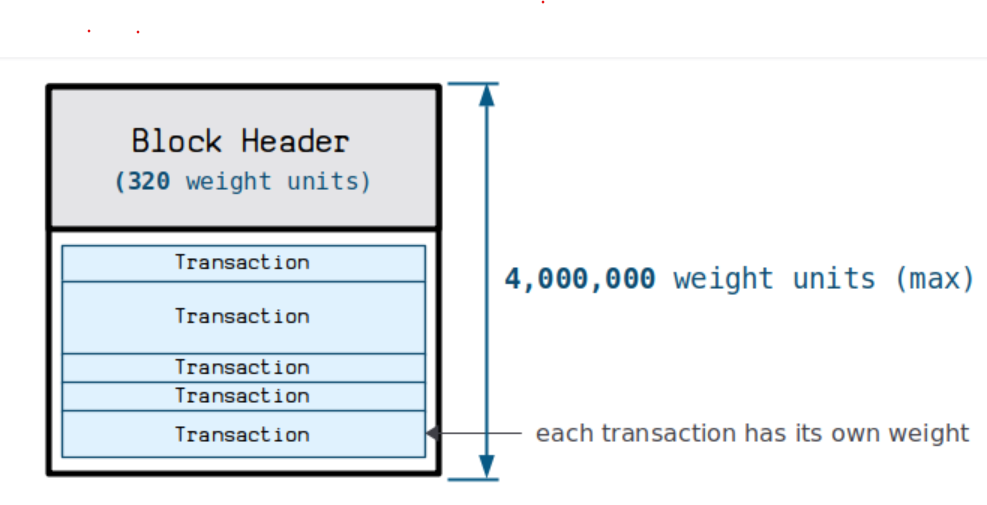
\includegraphics[width=0.85\columnwidth]{images/block-size.png} 
    \caption{Block size}
    \label{fig:block-size}
\end{figure}

\subsubsection{transaction size}

The transaction size will be calculated as the following picture:

\begin{figure}[ht] 
    \centering  
    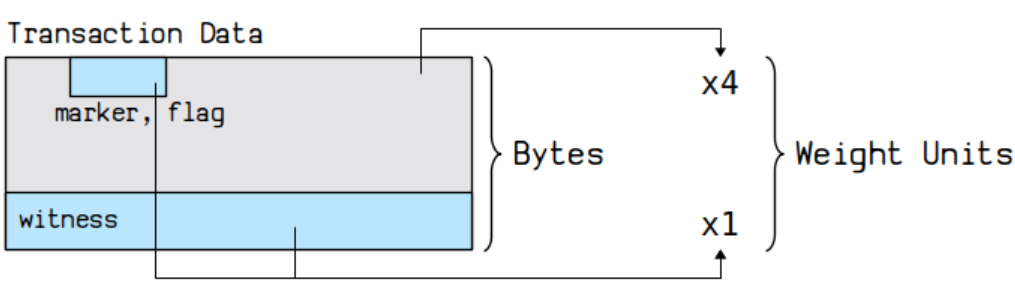
\includegraphics[width=0.85\columnwidth]{images/transaction-size.png} 
    \caption{Transaction size}
    \label{fig:transaction-size}
\end{figure}

You can check more details in \cite{website:transaction-size}


\subsection{Transaction constructure}

The transaction constructure of Bitcoin show in the following excel.

\begin{tabular}{|c|c|c|} \hline
    Field & Size & Description \\ \hline
    Version & 4 bytes & The version number for the transaction. Used to enable new features  \\ \hline
    \textcolor{blue}{Maker} & 1 bytes & Used to indicate a segwit transaction. Must be 00 \\ \hline
    \textcolor{blue}{Flag} & 1 bytes & Used to indicate a segwit transaction. Must be 01 or greater  \\ \hline
    Input Count & Variable & Indicates the number of inputs  \\ \hline
    Input-TXID & 32 bytes & The TXID of the transaction containing the output you want to spend  \\ \hline
    Input-VOUT & 4 bytes & The index number of the output you want to spend  \\ \hline
    Input-ScriptSig Size & Variable & The size in bytes of the upcoming ScriptSig  \\ \hline
    Input-ScriptSig & Variable & The unlocking code for the output you want to spend  \\ \hline
    Input-Sequnencer & 4 bytes & Set whether the transaction can be replaced or when it can be mined  \\ \hline
    Output Count & Variable & Indicates the number of outputs  \\ \hline
    Output-Amount & 8 bytes & The value of the output in satoshis  \\ \hline
    Output-ScriptPubKey Size & Variable & The size in bytes of the upcoming ScriptPubKey  \\ \hline
    Output-ScriptPubKey & Variable bytes & The locking code for this output  \\ \hline
    \textcolor{blue}{Witness-Stack Items} & Variable & The number of items to be pushed on to the stack as part of the unlocking code.  \\ \hline
    \textcolor{blue}{Witness-Stack Items-Size} & Variable & The size of the upcoming stack item  \\ \hline
    \textcolor{blue}{Witness-Stack Items-Item} & Variable & The data to be pushed on to the stack  \\ \hline
    Locktime & 4 bytes & Set a time or height after which the transaction can be mined  \\ \hline
\end{tabular}

The \textcolor{blue}{blue} part means it will be stored in segwit part. Any one could check more details in \cite{website:transaction-constructure}
    \section{Bench data} \label{sec:bench-data}

This section mainly give some bench datas for some operators used in Groth16 verification process.

\subsection{operators-script-size-origin}

We give some initial bench data we test in current implement first. Including:

\begin{itemize}
    \item Double and Add operators in $G_1$ group;
    \item Double and Add operators in $G_2$ group;
    \item Field operators in extension field;
\end{itemize}

\subsubsection{G1 group}

\begin{tabular}{|c|c|c|c|} \hline
operator typr & script size & max depth & exceed 4M? \\ \hline
$2 \cdot g_1$ & 1,752,916 bytes & 131 & no  \\ \hline
$g_1 \cdot g_1^{'}$ & 3,997,319 bytes &	< 1000 & no \\ \hline
\end{tabular}

\subsubsection{G2 group}

\begin{tabular}{|c|c|c|c|} \hline
operator typr & script size & max depth & exceed 4M? \\ \hline
$2 \cdot g_2$ & \textcolor{red}{7,019891} bytes & 815 & yes  \\ \hline
$g_2 \cdot g_2^{'}$ & \textcolor{red}{9,270,854} bytes &	293 & yes \\ \hline
\end{tabular}

\subsubsection{field}

\begin{tabular}{|c|c|c|c|} \hline
operator typr & script size & max depth & exceed 4M? \\ \hline
$F_{q12}: a + b$ & 6,644 bytes & 220 & no  \\ \hline
$F_{q12}: 2 * a$ & 6,793 bytes & 217 & no \\ \hline
$F_{q12}: a * b$ & \textcolor{red}{11,641,775} bytes & 545 & yes \\ \hline
$F_{q12}: mul\_fq6\_by\_nonresidue$ & 4,923 bytes &	146 & no \\ \hline
$F_{q12}: frobenius\_map(1)$ & \textcolor{red}{4,541,887} bytes & - & yes \\ \hline
$F_{q12}: frobenius\_map(2)$ & 2,224,363 bytes & - & yes \\ \hline
$F_{q12}: mul\_by\_034$ & \textcolor{red}{9,810,459} bytes &	- & yes \\ \hline
$F_{q12}: ell\_by\_constant$ & \textcolor{red}{9,525,050} bytes & 383 & yes \\ \hline
$F_{q6}: a * b$ & 3,873,847 bytes &	275 & no \\ \hline
$F_{q6}: frobenius\_map(1)$ & 1,518,206 bytes &	- & no \\ \hline
$F_{q6}: frobenius\_map(2)$ & 598,274 bytes & - & no \\ \hline
$F_{q6}: mul\_by\_01\_with\_1\_constant$ & 3,280,529 bytes & 221 & no \\ \hline
$F_{q6}: mul\_by\_fp2\_constant$ & 1,520,337 bytes & 101 & no \\ \hline
$F_{q6}: mul\_by\_01$ & 3,769,633 bytes & - & no \\ \hline
$F_{q6}: mul\_by\_fp2$ & 2,252,362 bytes &	167 & no \\ \hline
$F_{q2}: a * b$ & 750,883 bytes & 113 & no \\ \hline

\end{tabular}


\subsection{operators-script-size-optimization}

The less script chunks, the better. So before we split the big operators, we want to optimize them first. We will give our new
data first and then clarification the pricinple.

\begin{itemize}
    \item Double and Add operators in $G_1$ group;
    \item Double and Add operators in $G_2$ group;
    \item Field operators in extension field;
\end{itemize}

\subsubsection{G1 group}

\begin{tabular}{|c|c|c|c|} \hline
operator typr & script size & optimized script size & exceed 4M? \\ \hline
$2 \cdot g_1$ & 1,752,916 bytes & \textcolor{green}{1,251,319} bytes & no  \\ \hline
$g_1 \cdot g_1^{'}$ & 3,997,319 bytes &	\textcolor{green}{1,001,977} bytes & no \\ \hline
\end{tabular}

\subsubsection{G2 group}

\begin{tabular}{|c|c|c|c|} \hline
operator typr & script size & optimized script size & exceed 4M? \\ \hline
$2 \cdot g_2$ & \textcolor{red}{7,019891} bytes & \textcolor{green}{3,262,334} bytes & yes  \\ \hline
$g_2 \cdot g_2^{'}$ & \textcolor{red}{9,270,854} bytes & \textcolor{green}{2,761,898} bytes & yes \\ \hline
\end{tabular}

\subsubsection{field}

\begin{tabular}{|c|c|c|c|} \hline
operator typr & script size & max depth & exceed 4M? \\ \hline
$F_{q12}: a + b$ & 6,644 bytes & 220 & no  \\ \hline
$F_{q12}: 2 * a$ & 6,793 bytes & 217 & no \\ \hline
$F_{q12}: a * b$ & \textcolor{red}{11,641,775} bytes & 545 & yes \\ \hline
$F_{q12}: mul\_fq6\_by\_nonresidue$ & 4,923 bytes &	146 & no \\ \hline
$F_{q12}: frobenius\_map(1)$ & \textcolor{red}{4,541,887} bytes & - & yes \\ \hline
$F_{q12}: frobenius\_map(2)$ & 2,224,363 bytes & - & yes \\ \hline
$F_{q12}: mul\_by\_034$ & \textcolor{red}{9,810,459} bytes &	- & yes \\ \hline
$F_{q12}: ell\_by\_constant$ & \textcolor{red}{9,525,050} bytes & 383 & yes \\ \hline
$F_{q6}: a * b$ & 3,873,847 bytes &	275 & no \\ \hline
$F_{q6}: frobenius\_map(1)$ & 1,518,206 bytes &	- & no \\ \hline
$F_{q6}: frobenius\_map(2)$ & 598,274 bytes & - & no \\ \hline
$F_{q6}: mul\_by\_01\_with\_1\_constant$ & 3,280,529 bytes & 221 & no \\ \hline
$F_{q6}: mul\_by\_fp2\_constant$ & 1,520,337 bytes & 101 & no \\ \hline
$F_{q6}: mul\_by\_01$ & 3,769,633 bytes & - & no \\ \hline
$F_{q6}: mul\_by\_fp2$ & 2,252,362 bytes &	167 & no \\ \hline
$F_{q2}: a * b$ & 750,883 bytes & 113 & no \\ \hline

\end{tabular}



    \section{Split pricinple} \label{sec:split-pricinple}

We will mainly introduce why we select a manually way to split the ZKP verification script.

\subsection{automately}


\subsection{manually}


    \section{Optimization pricinple} \label{sec:optimization-pricinple}

We will mainly introduce how we recude the script of operators in $G_1$ and $G_2$.

\subsection{group-g1}

It needs more opcodes if we implement the double or add operator in $G_1$ directly because there are some divison operators which
is not bitcoin-friendly. We obey the rules proposed in paper On Proving pairing.


\subsubsection{Double}

\begin{itemize}
    \item Show that the pair ($\lambda$, $\mu$), indeed define a tangent through $T$ showing that $\displaystyle y_1 - \lambda x_{1} - mu = 0$ 
    and $\displaystyle 2\lambda y_1 = 3x_1^2$. This step is dominated by $2\tilde{m}$ and one $\tilde{s}$
    \item Compute $\lambda^2$ which is simple one $\tilde{s}$
    \item Compute $\displaystyle x_3 = \lambda^2-2x_1$ and $\displaystyle 2\lambda y_3 = -\mu - \lambda x_3$ which is dominated by computing $\lambda x_3$
\end{itemize}

\subsubsection{Add}

\begin{itemize}
    \item Show that the pair ($\lambda$, $\mu$), indeed define a tangent through $T$ showing that $\displaystyle y_1 - \lambda x_{1} - mu = 0$ 
    and $\displaystyle y_2 - \lambda x_{2} - mu = 0$. This step is dominated by $2\tilde{m}$
    \item Compute $\lambda^2$ which is simple one $\tilde{s}$
    \item Compute $\displaystyle x_3 = \lambda^2-x_1-x_2$ and $\displaystyle 2\lambda y_3 = -\mu - \lambda x_3$ which is dominated by computing $\lambda x_3$
\end{itemize}
\subsection{group-g2}

The unique difference between $G_1$ and $G_2$ is that $G_1$ is based on $F_q$ while $G_2$ is based on $F_{q2}$.

Based on this optimization, we reduce the size of Double and Add operator largely. So we dont need to split the Double and 
Add operations now. This is a big improvement.

Additionally, we also highly reduce the size of Double and Add operators in $G_1$ as well. Now, we can combine at most 3 randome operators
into one script chunk while before optimization, we only could combine 2 Double operators into 1 script chunk and only 1 Add operator for 1
script chunk. It reduce the number of script chunks for MSM part to around 1/3 directly. 

    \section{Split data} \label{sec:split-data}

We give the result directly how we split the script which the size exceeds the 4M limitation. As we showed in the \ref{sec:bench-data},

There only have some operations of $F_{q12}$ need to be split after we optimize the operations for $G_1$ and $G_2$

\begin{tabular}{|c|c|c|c|} \hline
    operator typr & script size & max depth & exceed 4M? \\ \hline
    $F_{q12}: a * b$ & \textcolor{red}{11,641,775} bytes & 545 & yes \\ \hline
    $F_{q12}: frobenius\_map(1)$ & \textcolor{red}{4,541,887} bytes & - & yes \\ \hline
    $F_{q12}: mul\_by\_034$ & \textcolor{red}{9,810,459} bytes & - & yes \\ \hline
    $F_{q12}: ell\_by\_constant$ & \textcolor{red}{9,525,050} bytes & 383 & yes \\ \hline    
\end{tabular}


We will show how we split these 4 big script one by one, as we split it manually, we try our best to satifying the following property cocurrently:

\begin{itemize}
    \item Doesn't exceed the limitation of size and stack depth;
    \item Keeping the size of input and output is minimal;
    \item Try our best to make logic of each chunk is readable; 
\end{itemize}

\subsection{split-code}

\lstdefinestyle{mystyle}{
    % backgroundcolor=\color{backcolour},		% 背景色   
    keywordstyle= \color{ blue!70},			% 关键字/程序语言中的保留字颜色
    commentstyle= \color{red!50!green!50!blue!50},		% 程序中注释的颜色
    % commentstyle= \color[RGB]{40, 400, 255}
    numberstyle=\tiny\color{codegray},		% 左侧行号显示的颜色
    stringstyle=\color{codepurple},
    basicstyle=\ttfamily\footnotesize,
    breakatwhitespace=false,         
    breaklines=true,		% 对过长的代码自动换行                
    captionpos=b,                    
    keepspaces=true,                 
    numbers=left,		% 在左侧显示行号                 
    numbersep=5pt,                  
    showspaces=false,                
    showstringspaces=false,		% 不显示字符串中的空格
    showtabs=false,                  
    tabsize=2,
    % frame=none,		% 不显示边框
    frame=shadowbox,	% 边框阴影
    %   escapebegin=\begin{CJK*},escapeend=\end{CJK*},      % 代码中出现中文必须加上,否则报错
}

\subsubsection{$F_{q12} : a \cdot b$}

\begin{lstlisting}

    % Split Fq12 mul into small scripts. For each script
    % size < 4M && max_stack_used < 1000
    % Input: a0, a1, b0, b1
    %
    % Algorithm:
    %     Final_a0 = a0 * b0 + a1 * b1 * \gamma
    %     Final_a1 = (a0 + a1) * (b0 + b1) - (a0 * b0 + a1 * b1)
    pub fn split_mul() -> Vec<Script> {
        % The degree-12 extension on BN254 Fq6 is under the polynomial z^2 - y

        let mut res = vec![];

        res.push(script! {
            % a0, b0
            { Fq6::mul(6, 0) }
            % a0 * b0
        });

        res.push(script! {
            % a1, b1
            { Fq6::mul(6, 0) }
            % a1 * b1
        });

        res.push(script! {
            % a0 * b0, a1 * b1, a0, a1, b0, b1,
            { Fq6::add(6, 0) }
            % a0 * b0, a1 * b1, a0, a1, b0 + b1,
            { Fq6::add(12, 6) }
            % a0 * b0, a1 * b1, b0 + b1, a0 + a1,
            { Fq6::mul(6, 0) }
            % a0 * b0, a1 * b1, (a0 + a1) * (b0 + b1)
            { Fq6::copy(12) }
            % a0 * b0, a1 * b1, (a0 + a1) * (b0 + b1), a0 * b0
            { Fq6::copy(12) }
            % a0 * b0, a1 * b1, (a0 + a1) * (b0 + b1), a0 * b0, a1 * b1
            { Fq12::mul_fq6_by_nonresidue() }
            % a0 * b0, a1 * b1, (a0 + a1) * (b0 + b1), a0 * b0, a1 * b1 * \gamma
            % z^2 - \gamma = 0
            { Fq6::add(6, 0) }
            % a0 * b0, a1 * b1, (a0 + a1) * (b0 + b1), a0 * b0 + a1 * b1 * \gamma
            { Fq6::add(18, 12)}
            % (a0 + a1) * (b0 + b1), a0 * b0 + a1 * b1 * \gamma, a0 * b0 + a1 * b1
            { Fq6::sub(12, 0) }
            % a0 * b0 + a1 * b1 * \gamma, (a0 + a1) * (b0 + b1) - (a0 * b0 + a1 * b1)
        });

        res
    }

\end{lstlisting}

\subsubsection{$F_{q12} : frobenius\_map(1)$}

\begin{lstlisting}

    pub fn split_frobenius_map(i: usize) -> Vec<Script> {
        let mut res = vec![];
        if i == 1 {
            % [p.c0, p.c1]
            res.push(script! {
                { Fq6::frobenius_map(i) }
                { Fq6::roll(6) }
                { Fq6::frobenius_map(i) }
                % [p.c1 ^ p^i, p.c0 ^ p^i]
            });
            % [p.c1 ^ p^i]
            res.push(Fq6::mul_by_fp2_constant(
                &ark_bn254::Fq12Config::FROBENIUS_COEFF_FP12_C1
                    [i % ark_bn254::Fq12Config::FROBENIUS_COEFF_FP12_C1.len()],
            ));
        } else {
            res.push(Self::frobenius_map(i));
        }

        res
    }
\end{lstlisting}

\subsubsection{$F_{q12}: mul\_by\_034$}

\begin{lstlisting}

    pub fn split_mul_by_034() -> Vec<Script> {
        let mut res = vec![];

        % compute b = p.c1 * (c3, c4)
        % [p.c1, c3, c4]
        res.push(Fq6::mul_by_01());
        % [b]

        % [c0, c3, b, p.c0, p.c1]
        % [Fq2, Fq2, Fq6, Fq6, Fq6]
        res.push(script! {
            % compute a = c0 * p.c0
            { Fq6::copy(6) }
            % [c0, c3, b, p.c0, p.c1, p.c0]
            { Fq2::copy(26) }
            % [c0, c3, b, p.c0, p.c1, p.c0, c0]
            { Fq6::mul_by_fp2() }
            % [c0, c3, b, p.c0, p.c1, c0 * p.c0]
            % [c0, c3, b, p.c0, p.c1, a]
            % compute gamma * b
            { Fq6::roll(18) }
            % [c0, c3, p.c0, p.c1, a, b]
            { Fq12::mul_fq6_by_nonresidue() }
            % [c0, c3, p.c0, p.c1, a, b * gamma]

            % compute final c0 = a + gamma * b
            % [c0, c3, p.c0, p.c1, a, b * gamma]
            { Fq6::copy(6) }
            % [c0, c3, p.c0, p.c1, a, b * gamma, a]
            { Fq6::add(6, 0) }
            % [c0, c3, p.c0, p.c1, a, a + b * gamma]
            % [c0, c3, p.c0, p.c1, a, final_c0]

            % compute e = p.c0 + p.c1
            { Fq6::add(18, 12) }
            % [c0, c3, a, final_c0, p.c0 + p.c1]
            % [c0, c3, a, final_c0, e]

            % compute c0 + c3
            { Fq2::add(20, 18) }
            % [a, final_c0, e, c0 + c3]
        });

        % [b, a, final_c0, e, c0 + c3, c4]
        res.push(script! {
            % update e = e * (c0 + c3, c4)
            { Fq6::mul_by_01() }
            % [b, a, final_c0, e]

            % sum a and b
            { Fq6::add(18, 12) }
            % [final_c0, e, b + a]

            % compute final c1 = e - (a + b)
            { Fq6::sub(6, 0) }
            % [final_c0, e - (b + a)]
            % [final_c0, final_c1]
        });

        res
    }
    
\end{lstlisting}


\subsubsection{$F_{q12}: mul\_by\_constant$}

\begin{lstlisting}

    pub fn split_mul_by_034_with_4_constant(constant: &ark_bn254::Fq2) -> Vec<Script> {
        let mut res = vec![];

        % [p.c1, c3], constant = c4
        res.push(Fq6::mul_by_01_with_1_constant(constant));

        % compute a = p.c0 * c0
        % Input: [p.c0, c0]
        % Output: [p.c0 * c0]
        res.push(Fq6::mul_by_fp2());

        % [c0, c3, p.c0, p.c1, a, b]
        res.push(script! {
            { Fq6::copy(0) }
            % [c0, c3, p.c0, p.c1, a, b, b]
            % compute beta * b
            { Fq12::mul_fq6_by_nonresidue() }
            % [c0, c3, p.c0, p.c1, a, b, b * beta]

            % compute final c0 = a + beta * b
            { Fq6::copy(12) }
            % [c0, c3, p.c0, p.c1, a, b, b * beta, a]
            { Fq6::add(6, 0) }
            % [c0, c3, p.c0, p.c1, a, b, a + beta * b]
            % [c0, c3, p.c0, p.c1, a, b, final_c0]

            % compute e = p.c0 + p.c1
            { Fq6::add(24, 18) }
            % [c0, c3, a, b, final_c0, e]

            % compute c0 + c3
            { Fq2::add(26, 24) }
            % [a, b, final_c0, e, c0 + c3]

            % update e = e * (c0 + c3, c4)
            { Fq6::mul_by_01_with_1_constant(constant) }
            % [a, b, final_c0, e]

            % sum a and b
            { Fq6::add(18, 12) }
            % [final_c0, e, a + b]

            % compute final c1 = e - (a + b)
            { Fq6::sub(6, 0) }
            % [final_c0, final_c1]
        });

        res
    }

\end{lstlisting}
\subsection{split-result}

We give the split result directly as follow excel:

\begin{tabular}{|c|c|c|c|c|} \hline
    operator typr & chunks & script size & max depth & exceed 4M? \\ \hline
    $F_{q12}: a * b$ & & \textcolor{red}{11,641,775} bytes & 545 & yes \\ \hline
     & chunk0 & \textcolor{green}{11,641,775} bytes & 545 & no \\ \hline
     & chunk1 & \textcolor{green}{11,641,775} bytes & 545 & no \\ \hline
     & chunk2 & \textcolor{green}{11,641,775} bytes & 545 & no \\ \hline
    $F_{q12}: frobenius\_map(1)$ & & \textcolor{red}{4,541,887} bytes & - & yes \\ \hline
    & chunk0 & \textcolor{green}{11,641,775} bytes & 545 & no \\ \hline
    & chunk1 & \textcolor{green}{11,641,775} bytes & 545 & no \\ \hline
    $F_{q12}: mul\_by\_034$ & & \textcolor{red}{9,810,459} bytes & - & yes \\ \hline
    & chunk0 & \textcolor{green}{11,641,775} bytes & 545 & no \\ \hline
    & chunk1 & \textcolor{green}{11,641,775} bytes & 545 & no \\ \hline
    & chunk2 & \textcolor{green}{11,641,775} bytes & 545 & no \\ \hline
    $F_{q12}: ell\_by\_constant$ & & \textcolor{red}{9,525,050} bytes & 383 & yes \\ \hline
    & chunk0 & \textcolor{green}{11,641,775} bytes & 545 & no \\ \hline
    & chunk1 & \textcolor{green}{11,641,775} bytes & 545 & no \\ \hline
    & chunk2 & \textcolor{green}{11,641,775} bytes & 545 & no \\ \hline
\end{tabular}

    \section{Next Steps}

Stay tuned for the next phase, featuring Fflonk \cite{website:Fflonk}, which is now integrated into the Polygon CDK \cite{website:Polygon-CDK}.

Some key metrics on Fflonk are as follows: 
\begin{itemize}
    \item Script size: 1.512292967 G
    \item Sub script numbers: 890
    \item Average script size: 1.699205 M
\end{itemize}
    

    \printbibliography[heading=bibintoc, title=\ebibname]
\end{document}
